\documentclass[11pt,]{article}
\usepackage[]{mathpazo}
\usepackage{amssymb,amsmath}
\usepackage{ifxetex,ifluatex}
\usepackage{fixltx2e} % provides \textsubscript
\ifnum 0\ifxetex 1\fi\ifluatex 1\fi=0 % if pdftex
  \usepackage[T1]{fontenc}
  \usepackage[utf8]{inputenc}
\else % if luatex or xelatex
  \ifxetex
    \usepackage{mathspec}
  \else
    \usepackage{fontspec}
  \fi
  \defaultfontfeatures{Ligatures=TeX,Scale=MatchLowercase}
\fi
% use upquote if available, for straight quotes in verbatim environments
\IfFileExists{upquote.sty}{\usepackage{upquote}}{}
% use microtype if available
\IfFileExists{microtype.sty}{%
\usepackage{microtype}
\UseMicrotypeSet[protrusion]{basicmath} % disable protrusion for tt fonts
}{}
\usepackage[margin=1in]{geometry}
\usepackage{hyperref}
\hypersetup{unicode=true,
            pdftitle={bluh},
            pdfauthor={Floor Komen},
            pdfkeywords={put some keywords here},
            pdfborder={0 0 0},
            breaklinks=true}
\urlstyle{same}  % don't use monospace font for urls
\usepackage{natbib}
\bibliographystyle{plainnat}
\usepackage{graphicx,grffile}
\makeatletter
\def\maxwidth{\ifdim\Gin@nat@width>\linewidth\linewidth\else\Gin@nat@width\fi}
\def\maxheight{\ifdim\Gin@nat@height>\textheight\textheight\else\Gin@nat@height\fi}
\makeatother
% Scale images if necessary, so that they will not overflow the page
% margins by default, and it is still possible to overwrite the defaults
% using explicit options in \includegraphics[width, height, ...]{}
\setkeys{Gin}{width=\maxwidth,height=\maxheight,keepaspectratio}
\IfFileExists{parskip.sty}{%
\usepackage{parskip}
}{% else
\setlength{\parindent}{0pt}
\setlength{\parskip}{6pt plus 2pt minus 1pt}
}
\setlength{\emergencystretch}{3em}  % prevent overfull lines
\providecommand{\tightlist}{%
  \setlength{\itemsep}{0pt}\setlength{\parskip}{0pt}}
\setcounter{secnumdepth}{0}
% Redefines (sub)paragraphs to behave more like sections
\ifx\paragraph\undefined\else
\let\oldparagraph\paragraph
\renewcommand{\paragraph}[1]{\oldparagraph{#1}\mbox{}}
\fi
\ifx\subparagraph\undefined\else
\let\oldsubparagraph\subparagraph
\renewcommand{\subparagraph}[1]{\oldsubparagraph{#1}\mbox{}}
\fi

%%% Use protect on footnotes to avoid problems with footnotes in titles
\let\rmarkdownfootnote\footnote%
\def\footnote{\protect\rmarkdownfootnote}

%%% Change title format to be more compact
\usepackage{titling}

% Create subtitle command for use in maketitle
\newcommand{\subtitle}[1]{
  \posttitle{
    \begin{center}\large#1\end{center}
    }
}

\setlength{\droptitle}{-2em}

  \title{bluh}
    \pretitle{\vspace{\droptitle}\centering\huge}
  \posttitle{\par}
    \author{Floor Komen}
    \preauthor{\centering\large\emph}
  \postauthor{\par}
      \predate{\centering\large\emph}
  \postdate{\par}
    \date{15 januari 2019}

\usepackage{booktabs}
\usepackage{longtable}
\usepackage{array}
\usepackage{multirow}
\usepackage[table]{xcolor}
\usepackage{wrapfig}
\usepackage{float}
\usepackage{colortbl}
\usepackage{pdflscape}
\usepackage{tabu}
\usepackage{threeparttable}
\usepackage{threeparttablex}
\usepackage[normalem]{ulem}
\usepackage{makecell}

\begin{document}
\maketitle
\begin{abstract}
Put the abstract over here
\end{abstract}

\section{2. Multiple linear
regression}\label{multiple-linear-regression}

In this chapter multiple linear models are generated. The demographics
tested in this model are the highly educated fraction in a municipality
\texttt{High\_educated\_frac}, the urban index of a municipality
\texttt{Urban\_index}, the mean income of the municipality
\texttt{Mean\_income}, the non-west factor \texttt{Non\_west} and the
fraction that is 60 plus in the municipality \texttt{Frac\_60plus}. The
error assumptions are also discussed. This are assumptions made for the
residuals, to check if meet the requirements for correct linear
regressions. These assumptions are: * Linearity: The expected value of
the error is zero * Constant variance: The variance of the error is
constant * Normality: The errors are normally distributed * Indepence:
The observations are sampled indipendently

\subsection{First model}\label{first-model}

The first model will be the model with all the demographics:\\
\(Y_i = \beta_0 + \beta_1*high educated fraction + \beta_2*Urban index + \beta_3*Mean income + \beta_4*Non west2 +\beta_5*Non west3 + \beta_6*Frac 60plus + \epsilon i\)\\
The outcome of this model is shown below:

\begin{table}[ht]
\centering
\begin{tabular}{rrrrr}
  \hline
 & Estimate & Std. Error & t value & Pr() \\ 
  \hline
(Intercept) & 0.3381 & 0.0314 & 10.78 & 0.0000 \\ 
  High\_educated\_frac & -0.0864 & 0.0454 & -1.90 & 0.0576 \\ 
  Urban\_index & -0.0193 & 0.0041 & -4.69 & 0.0000 \\ 
  Mean\_income & -0.0015 & 0.0011 & -1.46 & 0.1453 \\ 
  Non\_west2 & -0.0223 & 0.0065 & -3.45 & 0.0006 \\ 
  Non\_west3 & -0.0455 & 0.0095 & -4.77 & 0.0000 \\ 
  Frac\_60plus & -0.5904 & 0.1494 & -3.95 & 0.0001 \\ 
   \hline
\end{tabular}
\end{table}

The first model is the total model, \texttt{high\_educated\_frac} and
\texttt{Mean\_income} do not have a significant t-value. Before any
conclusions are made, the assumptions are checked via plots and the VIF
is checked. The VIF is the Variation Inflation Factor, it implies if
there is multicollinearity between two or more variables. The formula
for VIF is \(1/(1-R^2)\) and the thresholdvalue is 10. So values above
10 give signs of multicollinearity. As shown below none of the values
are above 10, so no signs of collinearity.

\begin{verbatim}
## High_educated_frac        Urban_index        Mean_income 
##           1.846691           3.355218           1.576931 
##           Non_west        Frac_60plus 
##           3.109682           1.285869
\end{verbatim}

\begin{verbatim}
## [1]  74 298
\end{verbatim}

\begin{figure}[H]

{\centering 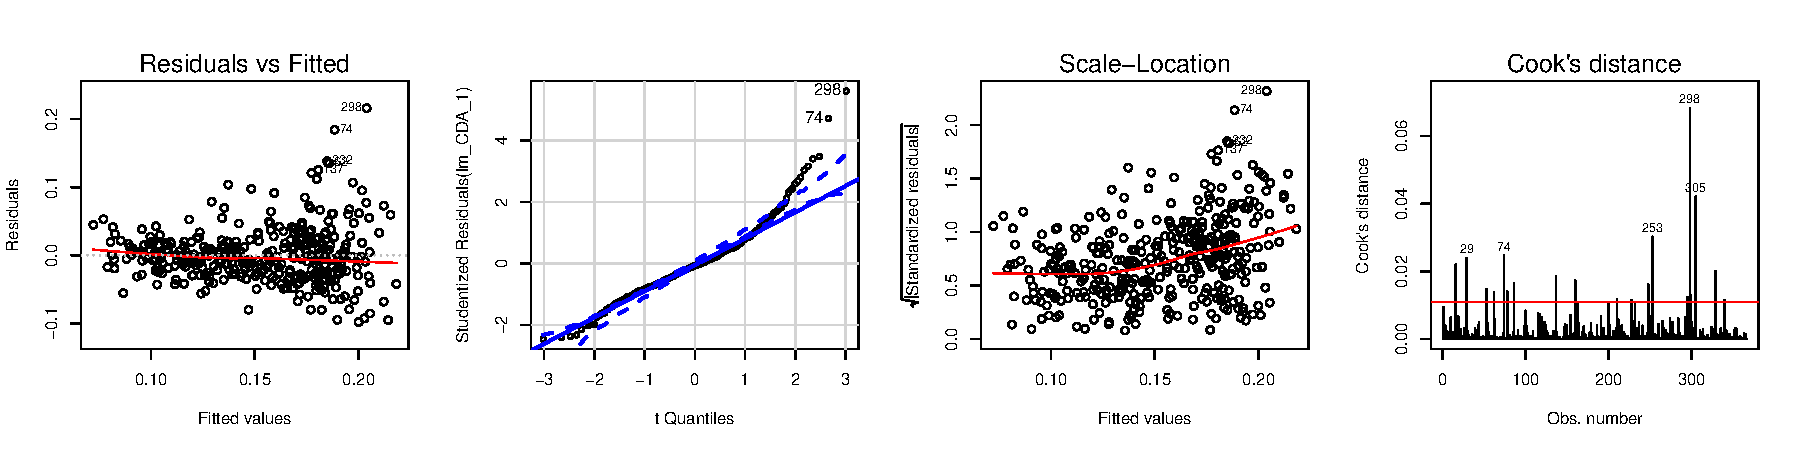
\includegraphics{lm_part_report_files/figure-latex/unnamed-chunk-1-1} 

}

\caption{\label{afm}assumptions first model}\label{fig:unnamed-chunk-1}
\end{figure}

In figure \ref{afm} the four plots are shown. The first plot (Residuals
vs Fitted) shows that the residuals have a `loudspeaker pattern', the
variance of the residuals tends to increase with an increase of the
fitted value. Because of this, a BoxCox graph is consulted. This graph
suggests a transformation for the response. The BoxCos figure \ref{BC1}
in has a 95\% Confidence interval located around the 0. So a ln
transformation is suggested.

\begin{figure}[H]

{\centering 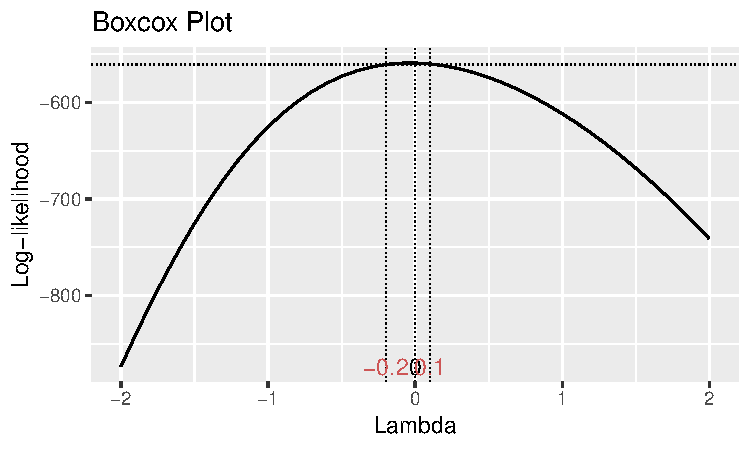
\includegraphics{lm_part_report_files/figure-latex/unnamed-chunk-2-1} 

}

\caption{\label{BC1}BoxCox first model}\label{fig:unnamed-chunk-2}
\end{figure}

\subsection{Second model}\label{second-model}

In the second model the response variable will be ln transformed. So the
new model will be:\\
\(ln(Y_i) = \beta_0 + \beta_1*high educated fraction + \beta_2*Urban index + \beta_3*Mean income + \beta_4*Non west2 + \beta_5*Non west 3 + \beta_6*Frac 60plus + \epsilon i\)

\begin{table}[ht]
\centering
\begin{tabular}{rrrrr}
  \hline
 & Estimate & Std. Error & t value & Pr() \\ 
  \hline
(Intercept) & -0.9944 & 0.1882 & -5.28 & 0.0000 \\ 
  High\_educated\_frac & -0.8808 & 0.2723 & -3.24 & 0.0013 \\ 
  Urban\_index & -0.1388 & 0.0247 & -5.62 & 0.0000 \\ 
  Mean\_income & -0.0024 & 0.0064 & -0.38 & 0.7042 \\ 
  Non\_west2 & -0.0991 & 0.0389 & -2.55 & 0.0112 \\ 
  Non\_west3 & -0.2763 & 0.0572 & -4.83 & 0.0000 \\ 
  Frac\_60plus & -2.6940 & 0.8965 & -3.01 & 0.0028 \\ 
   \hline
\end{tabular}
\end{table}

\begin{verbatim}
## [1]  16 298
\end{verbatim}

\begin{figure}[H]

{\centering 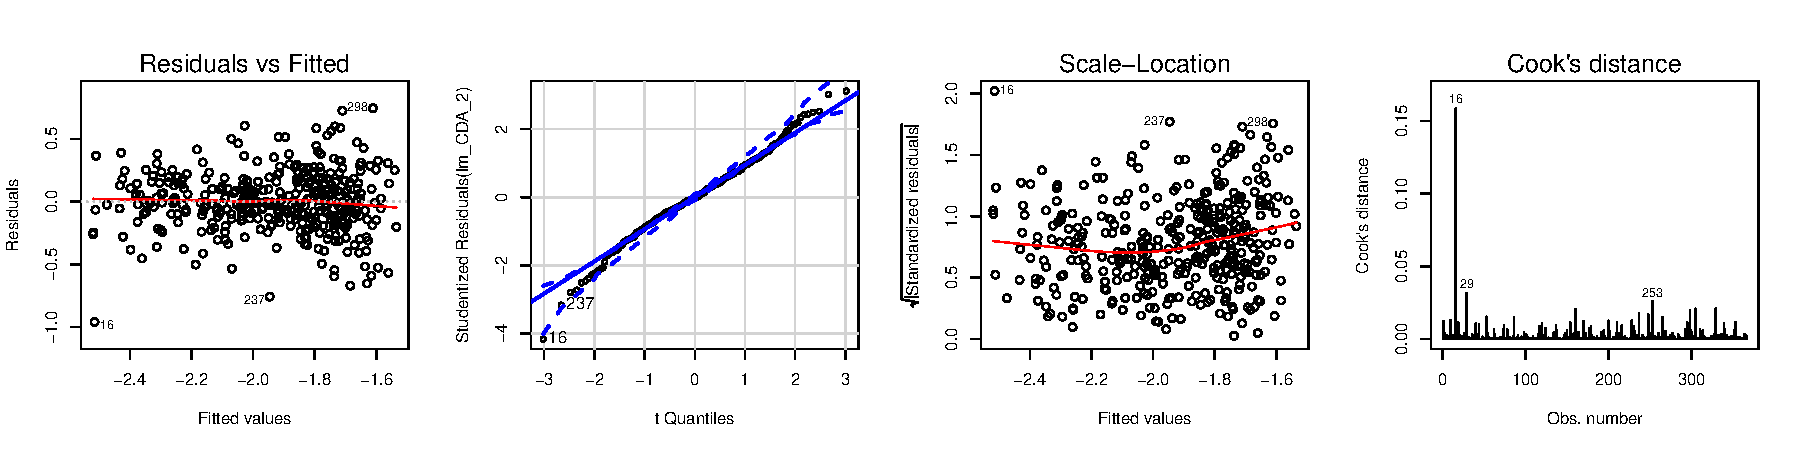
\includegraphics{lm_part_report_files/figure-latex/unnamed-chunk-3-1} 

}

\caption{\label{asm}assumptions second model}\label{fig:unnamed-chunk-3}
\end{figure}

The plots in figure \ref{asm} show one big outlier, the municipality
Amsterdam which has number 16. Amsterdams value for the cooks distance
goes way above the cutoff value for cooks, \(4/(369-5-1)=0.011\). It is
also outside the (-3,3) range with the studentized residuals. That is
why this municipality is removed.\\
For the second model without Amsterdam, a step function is used. This
step function uses the AIC for backward elimination. If the AIC can get
lower, because a variable is removed that variable will be removed else
no variable is removed. The formula for AIC is
\(AIC=-2log(likelihood)+2p\), p is the number of parameters in the
model. The variables that are left are the variables used in the final
model.

\begin{verbatim}
## Start:  AIC=-1042
## log(CDA_frac) ~ High_educated_frac + Urban_index + Mean_income + 
##     Non_west + Frac_60plus
## 
##                      Df Sum of Sq    RSS     AIC
## - Mean_income         1   0.02142 20.354 -1043.6
## <none>                            20.333 -1042.0
## - High_educated_frac  1   0.40428 20.737 -1036.8
## - Frac_60plus         1   0.64967 20.982 -1032.5
## - Non_west            1   1.45896 21.792 -1018.7
## - Urban_index         1   1.67178 22.005 -1015.2
## 
## Step:  AIC=-1043.61
## log(CDA_frac) ~ High_educated_frac + Urban_index + Non_west + 
##     Frac_60plus
## 
##                      Df Sum of Sq    RSS     AIC
## <none>                            20.354 -1043.6
## - Frac_60plus         1   0.64626 21.000 -1034.2
## - High_educated_frac  1   0.83927 21.193 -1030.9
## - Non_west            1   1.44891 21.803 -1020.5
## - Urban_index         1   1.65046 22.005 -1017.2
\end{verbatim}

\begin{verbatim}
## 
## Call:
## lm(formula = log(CDA_frac) ~ High_educated_frac + Urban_index + 
##     Non_west + Frac_60plus, data = Data_CDA[-16, ])
## 
## Coefficients:
##        (Intercept)  High_educated_frac         Urban_index  
##            -0.8921             -0.8199             -0.1294  
##           Non_west         Frac_60plus  
##            -0.1410             -2.9719
\end{verbatim}

\subsection{Final model}\label{final-model}

The backward elimination gave the final model.\\
\(ln(Y_i) = \beta_0 + \beta_1*high educated fraction + \beta_2*Urban index + \beta_4*Non west2 + \beta_5*Non west 3 + \beta_6*Frac 60plus + \epsilon i\)
The coëfficients are given in the table below

\begin{table}[ht]
\centering
\begin{tabular}{rrrrr}
  \hline
 & Estimate & Std. Error & t value & Pr($>$$|$t$|$) \\ 
  \hline
(Intercept) & -1.0298 & 0.1365 & -7.54 & 0.0000 \\ 
  High\_educated\_frac & -0.8277 & 0.2129 & -3.89 & 0.0001 \\ 
  Urban\_index & -0.1311 & 0.0240 & -5.46 & 0.0000 \\ 
  Non\_west2 & -0.1141 & 0.0378 & -3.02 & 0.0027 \\ 
  Non\_west3 & -0.2871 & 0.0559 & -5.13 & 0.0000 \\ 
  Frac\_60plus & -3.0168 & 0.8799 & -3.43 & 0.0007 \\ 
   \hline
\end{tabular}
\end{table}

\begin{verbatim}
## 237 298 
## 236 297
\end{verbatim}

\begin{figure}[H]

{\centering 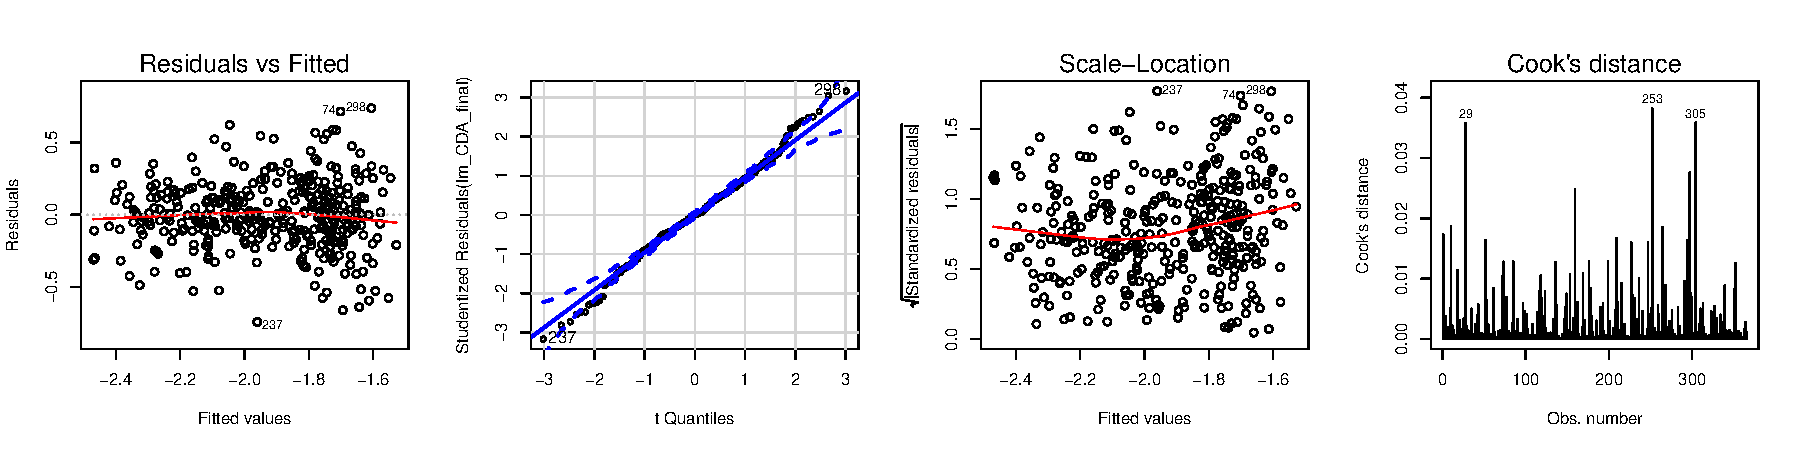
\includegraphics{lm_part_report_files/figure-latex/unnamed-chunk-5-1} 

}

\caption{\label{asm}assumptions second model}\label{fig:unnamed-chunk-5}
\end{figure}

The estimates for the predictors are filled in the model and the
following results are obtained:

\(ln(Y_i) = -1.0298 -0.8277*high educated fraction -0.1311*Urban index -0.1141*Non west2 -0.2871*Non west3 -3.0168*Frac 60plus + \epsilon i\)

All the coëfficients are negative, but because the fitted value is a log
value it will be positive.

\subsection{Cross validation}\label{cross-validation}


\end{document}
